\documentclass[a4paper, 11pt]{article}           %{{{1
% basic packages                                  {{{2
\usepackage[T1]{fontenc}
\usepackage[scaled=0.975]{helvet}
\usepackage[utf8]{inputenc}
\usepackage{amsmath}
\usepackage{lastpage}
\usepackage{graphicx}
\usepackage{amsfonts}
\usepackage{pgf,tikz}           % dessin
\usepackage{calc}           % calcul de longueur
\usepackage{multicol}
\usepackage{color}
\usepackage{tcolorbox}                                                          % encadrement texte
\usepackage{listings}                                                           %
% listings                                        {{{3
\definecolor{mygreen}{rgb}{0,0.6,0}
\definecolor{mygray}{rgb}{0.5,0.5,0.5}
\definecolor{mymauve}{rgb}{0.58,0,0.82}
\definecolor{deepblue}{rgb}{0,0,0.5}
\definecolor{deepred}{rgb}{0.6,0,0}
\definecolor{deepgreen}{rgb}{0,0.5,0}
\lstset{%
% backgroundcolor=\color{white},   % choose the background color; you must add \usepackage{color} or \usepackage{xcolor}; should come as last argument
basicstyle=\footnotesize,        % the size of the fonts that are used for the code
% breakatwhitespace=false,         % sets if automatic breaks should only happen at whitespace
% breaklines=true,                 % sets automatic line breaking
% captionpos=b,                    % sets the caption-position to bottom
commentstyle=\color{mygreen},    % comment style
% deletekeywords={type},           % if you want to delete keywords from the given language
% emph={},                         % Custom highlighting
% emphstyle=\ttb\color{deepred}    % Custom highlighting style
% escapeinside={\%*}{*)},          % if you want to add LaTeX within your code
% extendedchars=true,              % lets you use non-ASCII characters; for 8-bits encodings only, does not work with UTF-8
frame=shadowbox,                 % adds a frame around the code {single, shadowbox}
% keepspaces=true,                 % keeps spaces in text, useful for keeping indentation of code (possibly needs columns=flexible)
keywordstyle=\color{blue},       % keyword style
language=C,                      % the language of the code {Python, C}
% morekeywords={*,...},            % if you want to add more keywords to the set
numbers=left,                    % numbers = (none, left, right)
% numbersep=5pt,                   % how far the line-numbers are from the code
% numberstyle=\tiny\color{mygray}, % the style that is used for the line-numbers
% otherkeywords={self},            % Add keywords here
% rulecolor=\color{black},         % if not set, the frame-color may be changed on line-breaks within not-black text (e.g. comments (green here))
rulesepcolor=\color{gray}        % shadowbox color
% showspaces=false,                % show spaces everywhere adding particular underscores; it overrides 'showstringspaces'
% showstringspaces=false,          % underline spaces within strings only
% showtabs=false,                  % show tabs within strings adding particular underscores
% stepnumber=1,                    % the step between two line-numbers. If it's 1, each line will be numbered
% stringstyle=\color{mymauve},     % string literal style
% tabsize=4,                       % sets default tabsize to 2 spaces
% title=\lstname                   % show the filename of files included with \lstinputlisting; also try caption instead of title
}
%}}}
%}}}

% mise en page                                    {{{2
\addtolength{\voffset}{-1.8cm}
\addtolength{\textheight}{4cm}
\addtolength{\hoffset}{-2.5cm}
\addtolength{\textwidth}{4cm}
\addtolength{\headsep}{-0.5cm}
\usepackage{fancyhdr}
\setlength{\headheight}{14.00pt}
\pagestyle{fancy} % Numérotation des pages
\renewcommand\headrulewidth{1pt}
\fancyhead[L]{BP SN}
\fancyhead[C]{arduino}
\fancyhead[R]{entrée-sortie}
\renewcommand\footrulewidth{1pt}
\fancyfoot[L]{v 1.0 -- JB}
\fancyfoot[C]{\textbf{domotique, syst. embarqués \& de gestion de l'habitat}}
\fancyfoot[R]{\thepage/\pageref{LastPage}}
%\lhead{3E}%haut de page gauche
%}}}

% Compteurs:                                     {{{2
\addtocounter{page}{0}
\newcounter{Q}
\newcounter{exoNB}
%}}}

% newcommand                                     {{{2
\newcommand{\objectif}[1]{\textsc{\huge \textbf{Objectif :}\\ #1} }
\newcommand{\partie}[1]{\textsc{\Large #1} }
\newcommand{\question}{\stepcounter{Q} $\boxed{\arabic{Q}}$ }
\newcommand{\ligne}{\underline{\hspace{ \textwidth}} }
\newcommand{\LIGNE}{\vspace{2mm}\underline{\hspace{ \textwidth}} }
\newcommand{\reponse}{
  \par\nobreak
  \noindent\rule{0pt}{1.5\baselineskip}% Provides a larger gap between the preceding paragraph and the dots
  {\noindent\makebox[\linewidth]{\dotfill}\endgraf}% ... dotted lines ...
% \bigskip% Gap between dots and next paragraph
  }
\newcommand{\exo}[1]{\stepcounter{exoNB}\textsc{\Large Exercice \arabic{exoNB} -- #1} }
\newcommand{\EXO}[2]{\stepcounter{exoNB}\textsc{\Large Exercice \arabic{exoNB} -- #1} \hfill \textbf{#2 points}}
\newcommand{\pb}[1] {\stepcounter{exoNB}\textsc{\Large Problème \arabic{exoNB} -- #1} }
\newcommand{\PB}[2] {\stepcounter{exoNB}\textsc{\Large Problème \arabic{exoNB} -- #1} \hfill \textbf{#2 points}}
%}}}

% Longueur:                                      {{{2
\newlength{\longueurA}
\newlength{\longueurB}
\setlength{\parindent}{0pt}
\setlength{\parskip}{2pt}
\renewcommand{\baselinestretch}{1}
%}}}

% Divers                                          {{{2
% listings                                        {{{3
%\definecolor{mygreen}{rgb}{0,0.6,0}
%\definecolor{mygray}{rgb}{0.5,0.5,0.5}
%\definecolor{mymauve}{rgb}{0.58,0,0.82}
%\definecolor{deepblue}{rgb}{0,0,0.5}
%\definecolor{deepred}{rgb}{0.6,0,0}
%\definecolor{deepgreen}{rgb}{0,0.5,0}
%\lstset{%
%        backgroundcolor=\color{white},   % choose the background color; you must add \usepackage{color} or \usepackage{xcolor}; should come as last argument
%        basicstyle=\footnotesize,        % the size of the fonts that are used for the code
%        breakatwhitespace=false,         % sets if automatic breaks should only happen at whitespace
%        breaklines=true,                 % sets automatic line breaking
%        captionpos=b,                    % sets the caption-position to bottom
%        commentstyle=\color{mygreen},    % comment style
%        deletekeywords={...},            % if you want to delete keywords from the given language
%        escapeinside={\%*}{*)},          % if you want to add LaTeX within your code
%        extendedchars=true,              % lets you use non-ASCII characters; for 8-bits encodings only, does not work with UTF-8
%        frame=single,                    % adds a frame around the code
%        keepspaces=true,                 % keeps spaces in text, useful for keeping indentation of code (possibly needs columns=flexible)
%        keywordstyle=\color{blue},       % keyword style
%        morekeywords={*,...},            % if you want to add more keywords to the set
%        numbers=left,                    % where to put the line-numbers; possible values are (none, left, right)
%        numbersep=5pt,                   % how far the line-numbers are from the code
%        numberstyle=\tiny\color{mygray}, % the style that is used for the line-numbers
%        rulecolor=\color{black},         % if not set, the frame-color may be changed on line-breaks within not-black text (e.g. comments (green here))
%        showspaces=false,                % show spaces everywhere adding particular underscores; it overrides 'showstringspaces'
%        showstringspaces=false,          % underline spaces within strings only
%        showtabs=false,                  % show tabs within strings adding particular underscores
%        stepnumber=2,                    % the step between two line-numbers. If it's 1, each line will be numbered
%        stringstyle=\color{mymauve},     % string literal style
%        tabsize=4,                       % sets default tabsize to 2 spaces
%        title=\lstname                   % show the filename of files included with \lstinputlisting; also try caption instead of title
%}
%\lstset{%
%        language=Python,                 % the language of the code
%        otherkeywords={self},            % Add keywords here
%        deletekeywords={type},           % if you want to delete keywords from the given language
%        emph={},                         % Custom highlighting
%        emphstyle=\ttb\color{deepred}    % Custom highlighting style
%}
%}}}

% PRL style line                                 {{{3
\newlength{\diamondrulelength}
\setlength{\diamondrulelength}{0.6\textwidth}
\newlength{\diamondrulethickness}
\setlength{\diamondrulethickness}{2pt}
\newcommand{\diamondrule}{\begin{center}\tikz{\fill[black] (0.5\diamondrulelength,0) -- (0,0.5\diamondrulethickness) -- (-0.5\diamondrulelength,0) -- (0,-0.5\diamondrulethickness) -- cycle;}\end{center}}
%}}}

% fixed with tabular                             {{{3
\usepackage{array}
\newcolumntype{L}[1]{>{\raggedright\let\newline\\\arraybackslash\hspace{0pt}}m{#1}}
\newcolumntype{C}[1]{>{\centering\let\newline\\\arraybackslash\hspace{0pt}}m{#1}}
\newcolumntype{R}[1]{>{\raggedleft\let\newline\\\arraybackslash\hspace{0pt}}m{#1}}
%}}}

%}}}
%}}}

\begin{document}
\sffamily
\hfill Nom : {\noindent\makebox[5cm]{\dotfill}\endgraf}
\objectif{introduction aux entrées-sorties d'un micro-controlleur}\\

% https://learn.adafruit.com/adafruit-arduino-lesson-6-digital-inputs/overview

\partie{Le matériel}\\ %{{{1
- Une carte UNO + environnement de programmation arduino\\
- Une carte de prototypage et une demi-douzaine de fils\\
- Deux boutons poussoirs\\
- Deux résitances de 200 ohm\\
- Deux LEDs

%\begin{figure}[!h]
%\begin{center}
%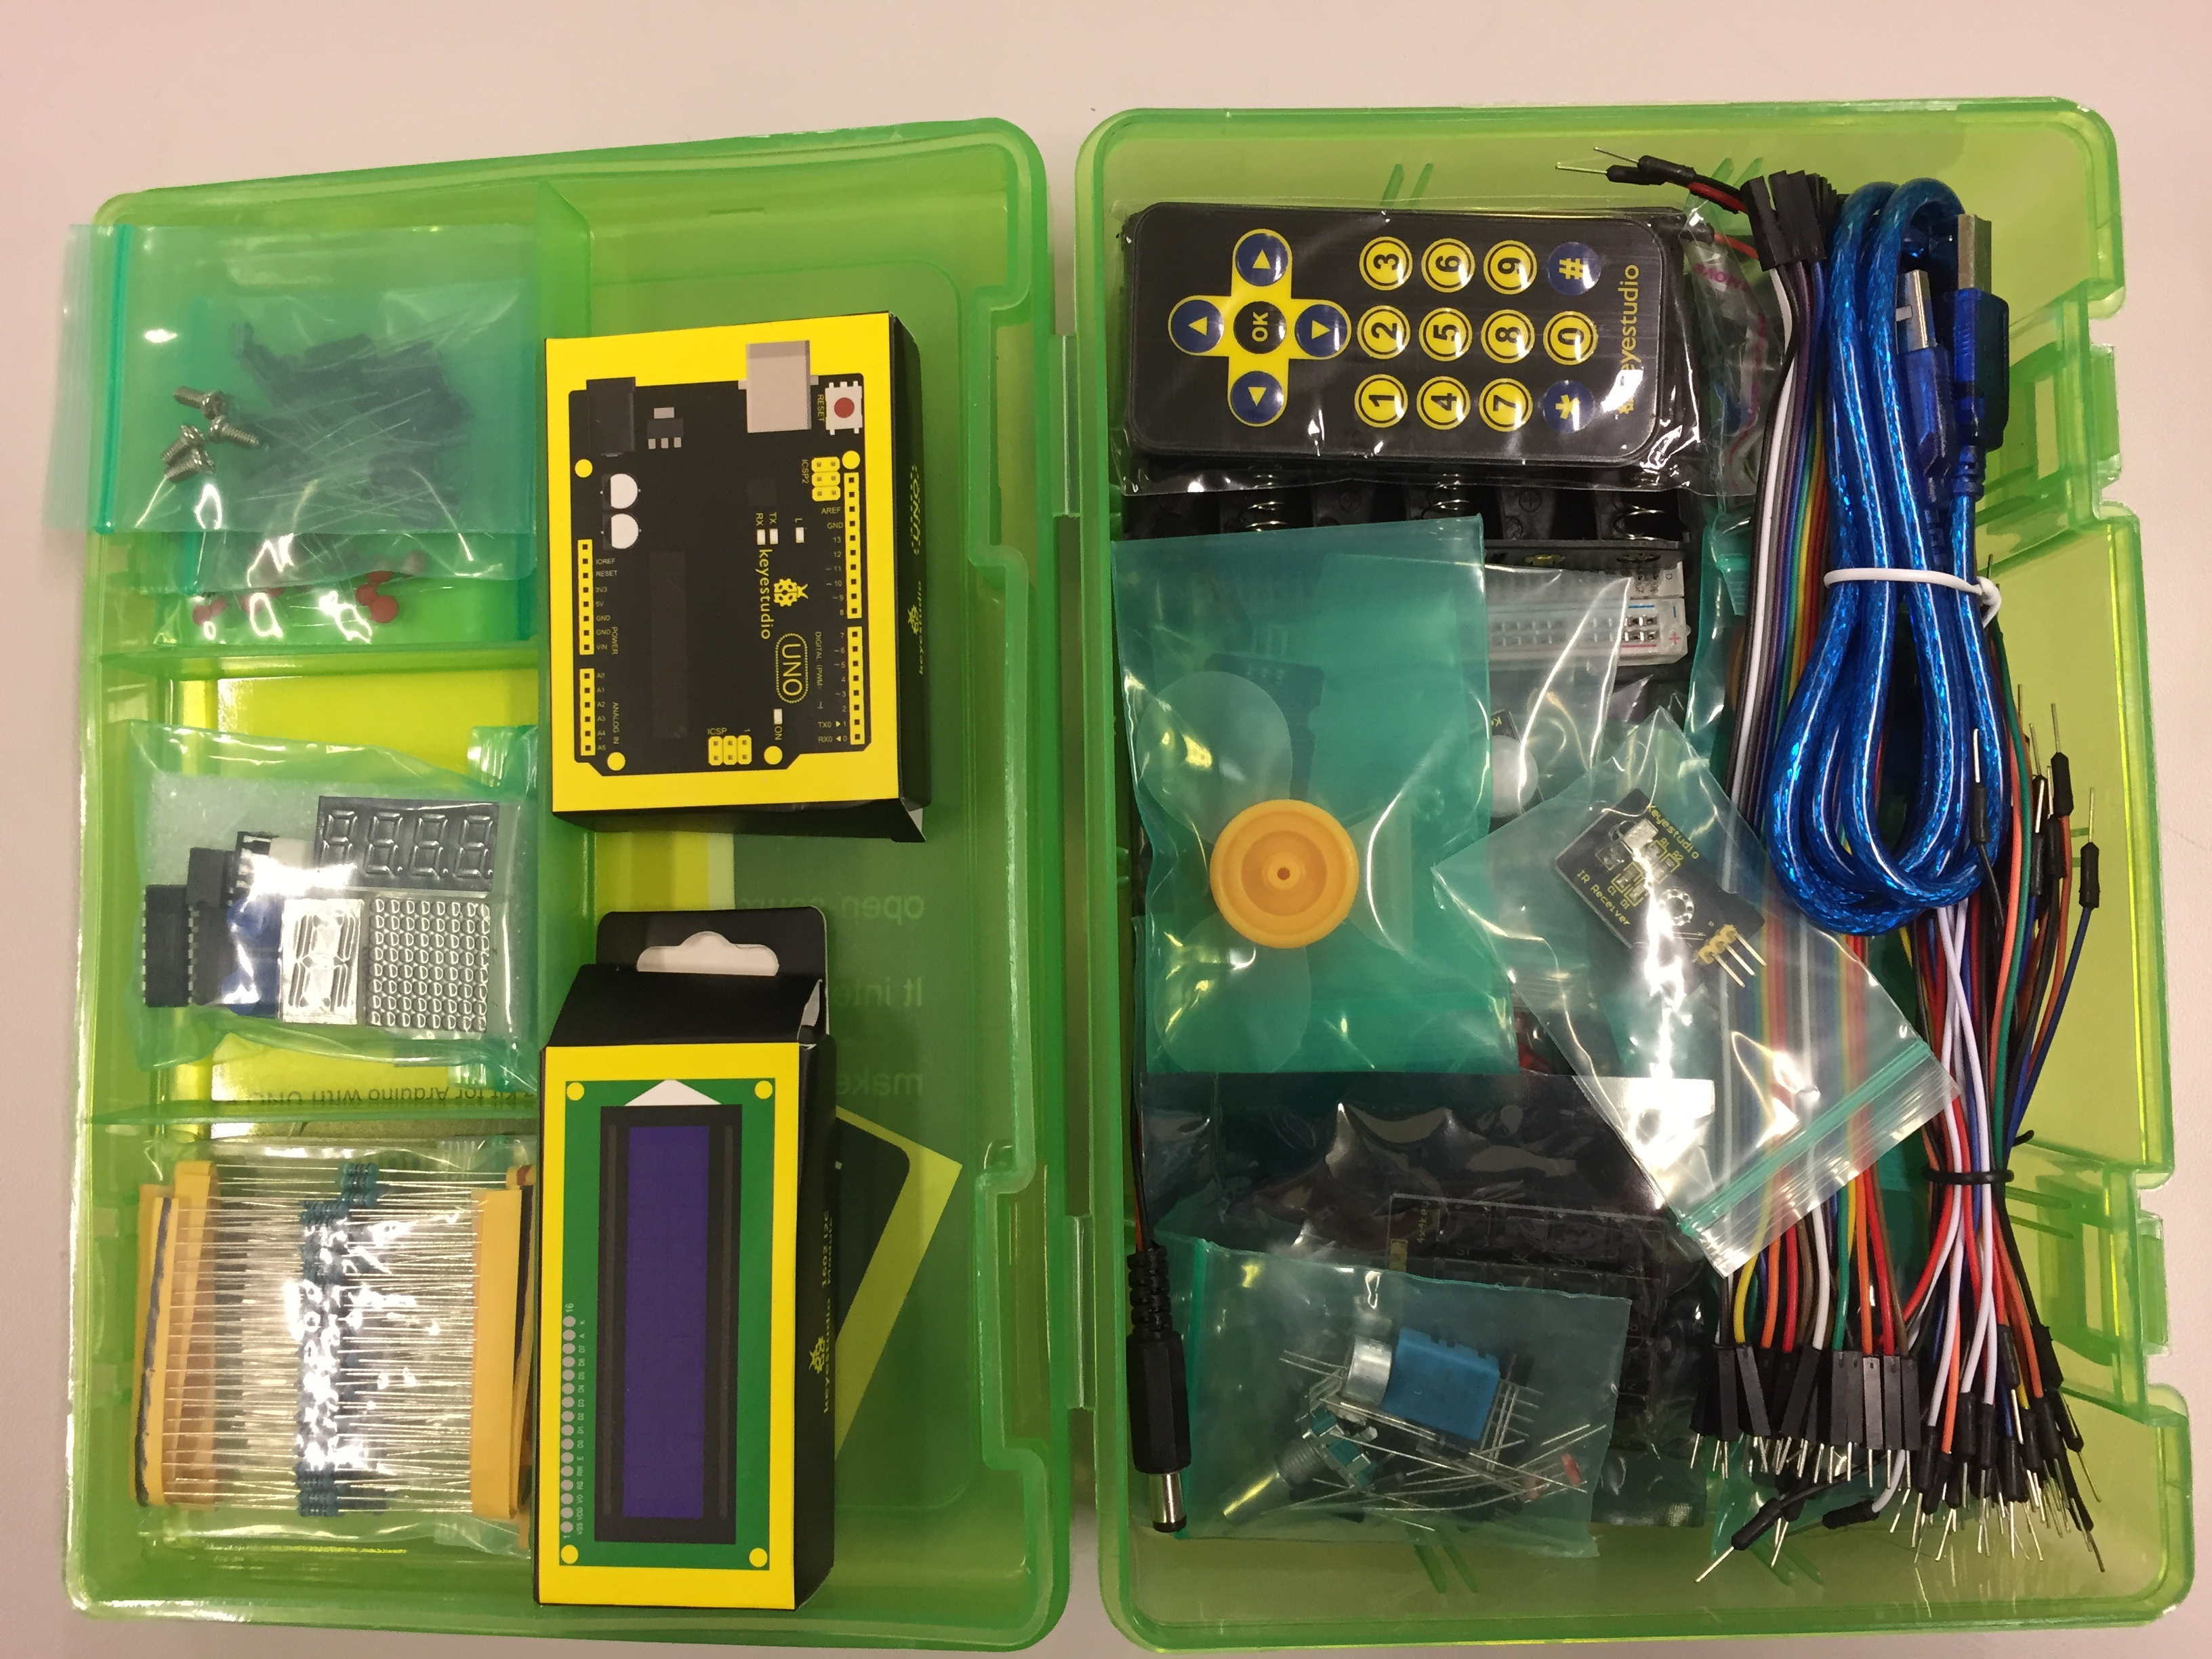
\includegraphics[width=0.75\textwidth]{coffret_arduino}\\
%\caption{Boite contenant le matériel listé ci-dessus. Le montage est dans la figure 2.}
%\end{center}
%\end{figure}
%}}}

\bigskip

\partie{Le bouton poussoir}\\ %{{{1
\begin{figure}[!b]
\begin{center}
\includegraphics[width=\textwidth]{CablageBouton}\\
\caption{La résistance série est d'envion 200 ohms.}
\end{center}
\end{figure}

\question Faire marcher le programme blink pour tester le bon fonctionnement de la carte et du téléversement. Au cas où ce programme était déjà dans le microcontrolleur, changez juste une instruction et vérifiez que le changement attendu se produit. J'aime faire clignoter la LED deux fois plus vite pour vérifier que ça marche comme je veux. Précisez les problèmes rencontrés, si tel est le cas.
\reponse

\question Ou est exécuté le programme ? Ou est-il stocké ?
\reponse

\question Réalisez le cablage de la figure "\textsc{Montage 1}". Précisez les difficultés rencontrées.
\reponse


\question La résistance série fait souvent environ 200 ohm, dans les conditions assez usuelles du montage. Décrivez comment trouver la valeur exacte de cette résistance série.
\reponse
\reponse
\reponse
\reponse

\question Une borne de la LED est reliée à une borne du bouton poussoir : ces deux bornes sont au même potentiel. Mesurez la tension entre ce potentiel et le potentiel de la masse. Quelle est la valeur de la tension quand la LED est allumée ? Eteinte ?
\reponse
\reponse
\tcbox{\textbf{Constatation professeur :} \hspace{5cm} }
%}}}

\bigskip

\partie{Entrée et sortie numériques}\\ %{{{1

\question Implémenter le code suivant et réaliser le montage montré dans les figure \ref{fig2bouton1} et \ref{fig2bouton2}.

\begin{lstlisting}
int ledPin = 5;
int buttonApin = 9;
int buttonBpin = 8;

byte leds = 0;

void setup() {
  pinMode(ledPin, OUTPUT);
  pinMode(buttonApin, INPUT_PULLUP);
  pinMode(buttonBpin, INPUT_PULLUP);
}

void loop() {
  if (digitalRead(buttonApin) == LOW) {
    digitalWrite(ledPin, HIGH);
  }
  if (digitalRead(buttonBpin) == LOW) {
    digitalWrite(ledPin, LOW);
  }
}
\end{lstlisting}

\begin{figure}
\begin{center}
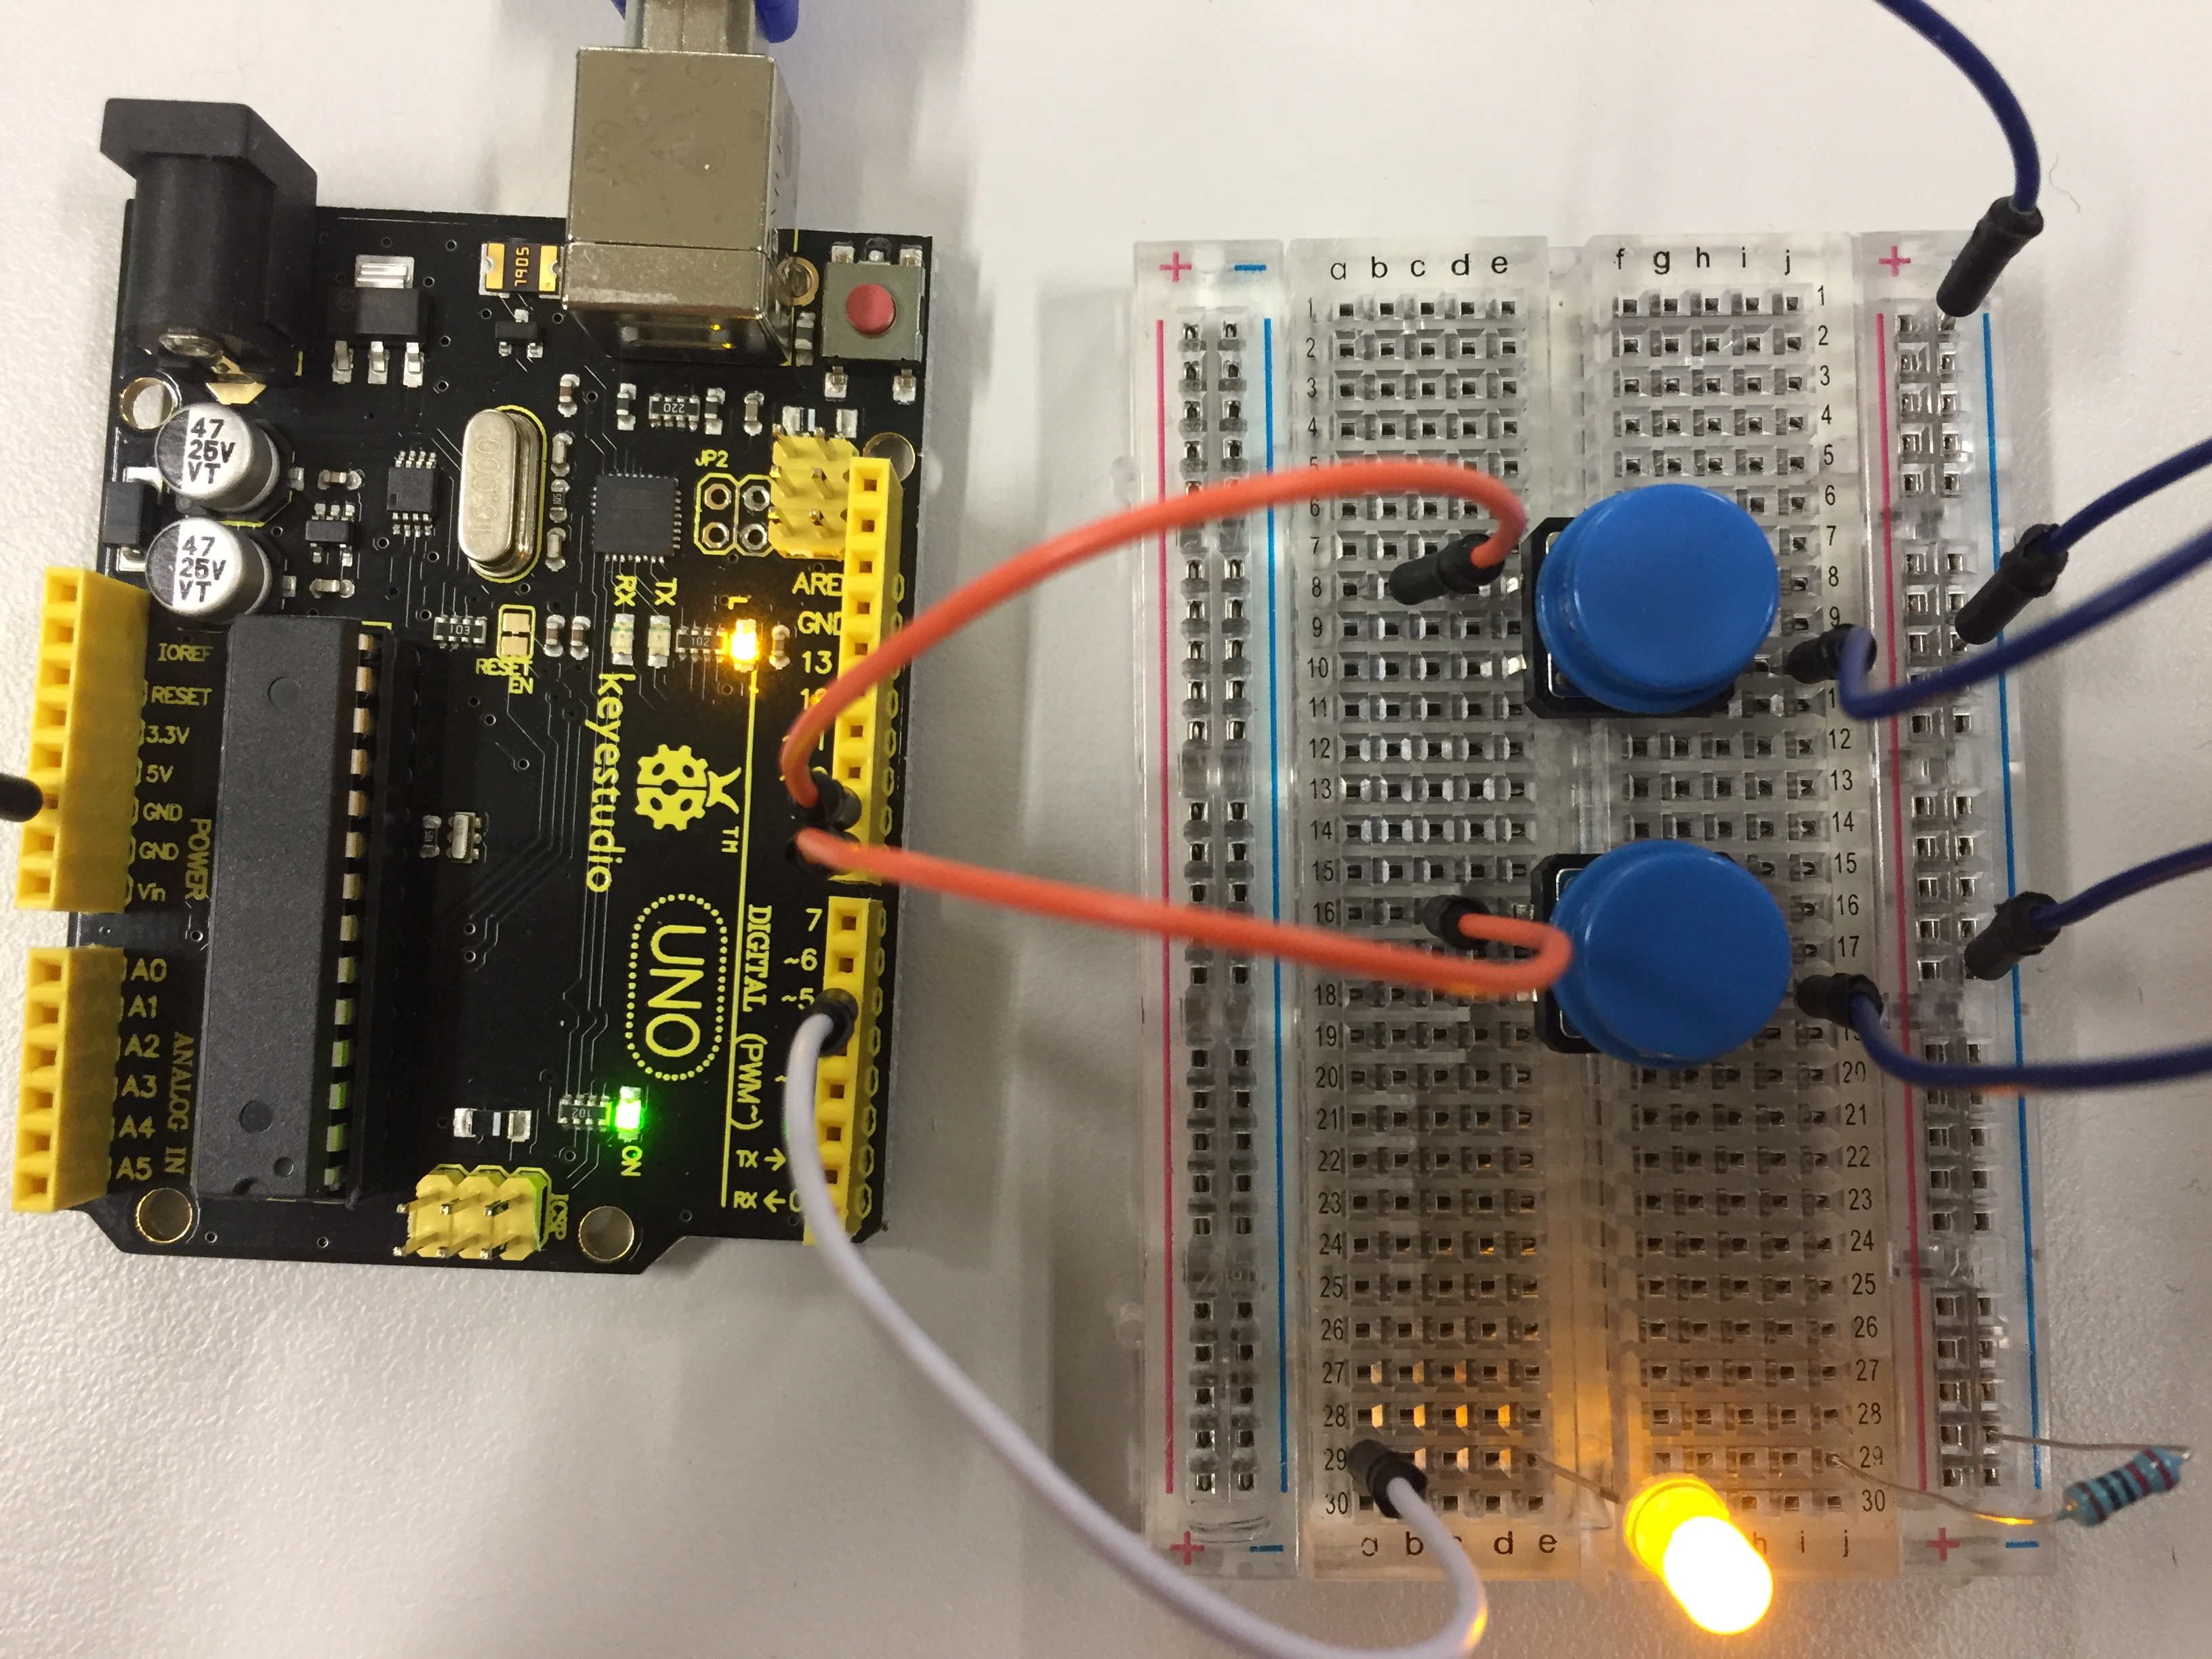
\includegraphics[width=0.85\textwidth]{deux_boutons}
\caption{Deux boutons sont lus par le micro-contrôleur. Montage.}
\label{fig2bouton1}
\end{center}
\end{figure}

\begin{figure}
\begin{center}
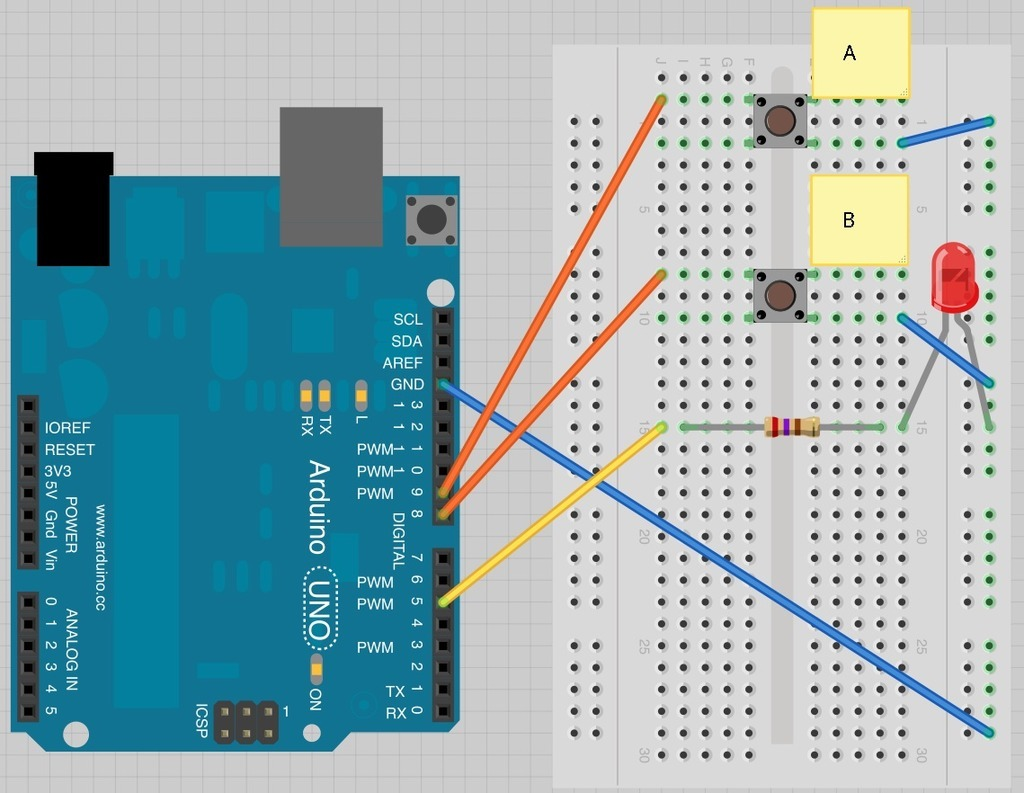
\includegraphics[width=0.85\textwidth]{cablage}\\
\caption{Deux boutons sont lus par le micro-contrôleur. Cablage.}
\label{fig2bouton2}
\end{center}
\end{figure}



\question Testez le montage et devinez ce que fait le programme ?
\reponse

\question Quels types\footnote{google : arduino type}\footnote{Datatype dans \texttt{https://www.arduino.cc/reference/en/} ; google translate peut être utile} ont les variables ledPin, buttonApin et buttonBpin ? A quoi ça sert de stocker ces nombres dans des variables ?
\reponse
\reponse

\question Combien de fois et quand est excécuté la fonction \texttt{setup()} ?
\reponse
\reponse

\question Combien de fois et quand est excécuté la fonction \texttt{loop}() ?
\reponse

\question Que se passe t'il lors de son excécution ? A quelle rapidité ?
\reponse
\reponse
\reponse

\question Qu'est ce que \texttt{INPUT PULLUP} ?
\reponse

\question S'il n'y avait pas la possibilité \texttt{INPUT PULLUP}, que ferait-on ? Peut-être qu'un schéma serait plus clair et concis.
\reponse
\vspace{2cm}

\question Sur les figures \ref{circuit1} et \ref{circuit2}, dessiner d'une part les potentiels lorsque le bouton est appuyé, on dira que le bouton est fermé. Et d'autre part lorsqu'il ne l'est pas, on dira que le bouton est ouvert. Préciser les potentiels des connections.
\begin{figure}
\begin{center}
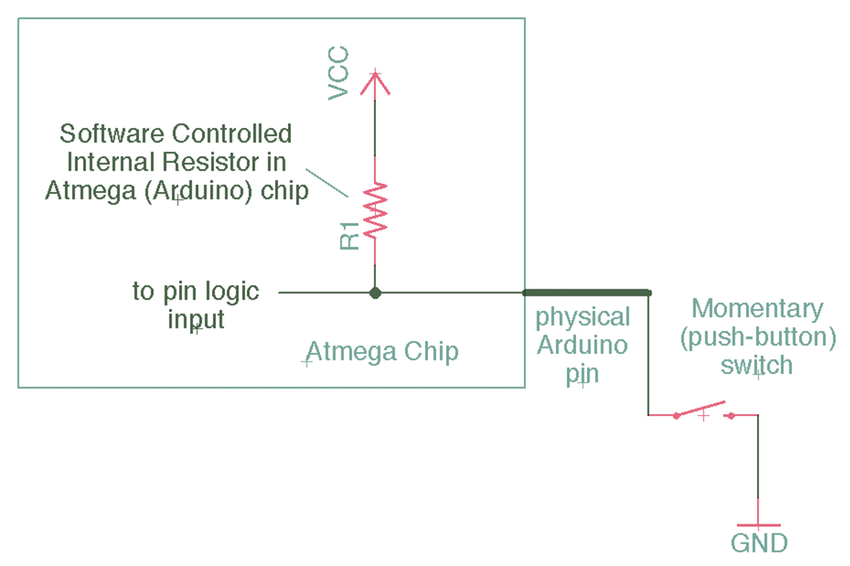
\includegraphics[width=0.6\textwidth]{input_pullup}\\
Circuit équivalent d'une entrée numérique du micro-controlleur ATMEGA 328.\\
\end{center}
\end{figure}

\begin{figure}
\begin{center}
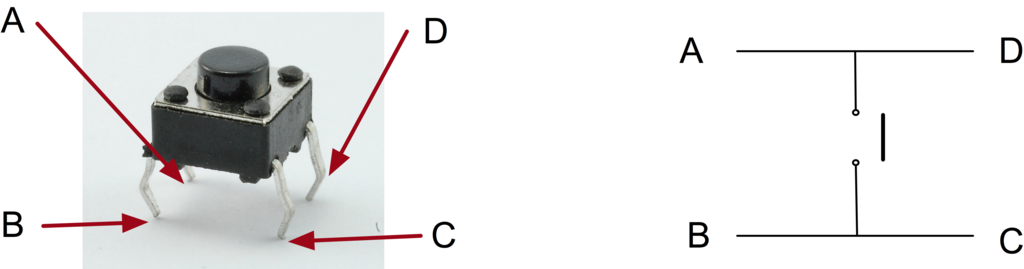
\includegraphics[width=0.6\textwidth]{switch}\\
\caption{Circuit équivalent des boutons poussoirs.%
Dessiner la résistance interne PULL-UP à l'arduino, avec sa valeur et la tension appliquée par l'arduino. Préciser la tension lue par l'entrée de l'arduino lorsque le bouton poussoir est \textbf{ouvert}.}
\label{circuit1}
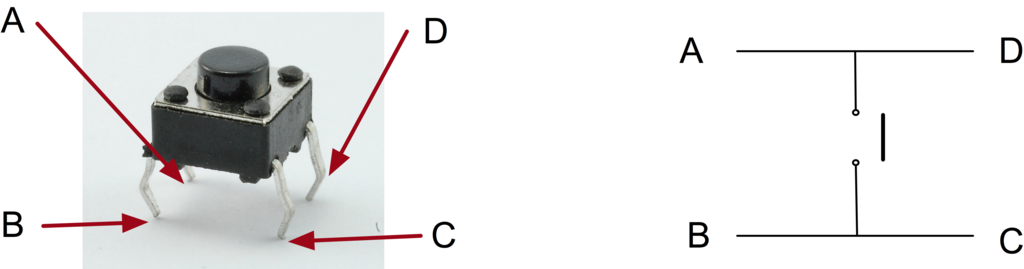
\includegraphics[width=0.6\textwidth]{switch}\\
\caption{Circuit équivalent des boutons poussoirs. Même question lorsque le bouton poussoir est \textbf{fermé}. De plus, modifier le bouton pour le représetner dans l'état fermé.}
\label{circuit2}
\end{center}
\end{figure}

\question Décrivez en une ou quelques phrases simples (décrire l'algorithme) la fonction \texttt{loop()}.
\reponse

\question Décrivez ce qui se passe lors de la fonction \texttt{setup()}.
\reponse
\tcbox{\textbf{Constatation professeur :} \hspace{5cm} }
%}}}

\bigskip

\partie{Entrée numérique et connexion série}\\ %{{{1


\begin{lstlisting}
int ledPin = 5;
int buttonApin = 9;
int buttonBpin = 8;

byte leds = 0;

void setup() {
  pinMode(ledPin, OUTPUT);
  pinMode(buttonApin, INPUT_PULLUP);
  pinMode(buttonBpin, INPUT_PULLUP);

  Serial.begin(9600);
}

void loop() {
  if (digitalRead(buttonApin) == LOW) {
    digitalWrite(ledPin, HIGH);
    Serial.println("bouton A presse");
  }
  if (digitalRead(buttonBpin) == LOW) {
    digitalWrite(ledPin, LOW);
    Serial.println("bouton B presse");
  }
}
\end{lstlisting}

\question Conservez le montage précédent et rajoutez une connection serie au programme en modifiant la source selon le code suivant :

\question Ouvrez le terminal série (voir figure \ref{TerminalSerie}) du logiciel arduino et décrivez ce que vous observez ?
\reponse

\tcbox{\textbf{Constatation professeur :} \hspace{5cm} }

\question En termes simples, à quoi sert la fonction \texttt{Serial.begin()} ?
\reponse

\question Quel est son argument ?
\reponse

\question En termes simples, à quoi sert la fonction \texttt{Serial.println()} ?
\reponse

\question Quel est son argument ?
\reponse

\question Quel retournent les fonctions \emph{(ou méthodes de l'objet Serial)} \texttt{Serial.println()} et \texttt{Serial.begin()} ? Est-ce utilisé ici ?
\reponse
\reponse

\question Pouvez vous écrire ici les lignes de codes ajoutées pour obtenir les valeurs retournées ?
\reponse
\reponse


\begin{figure}[!h]
\begin{center}
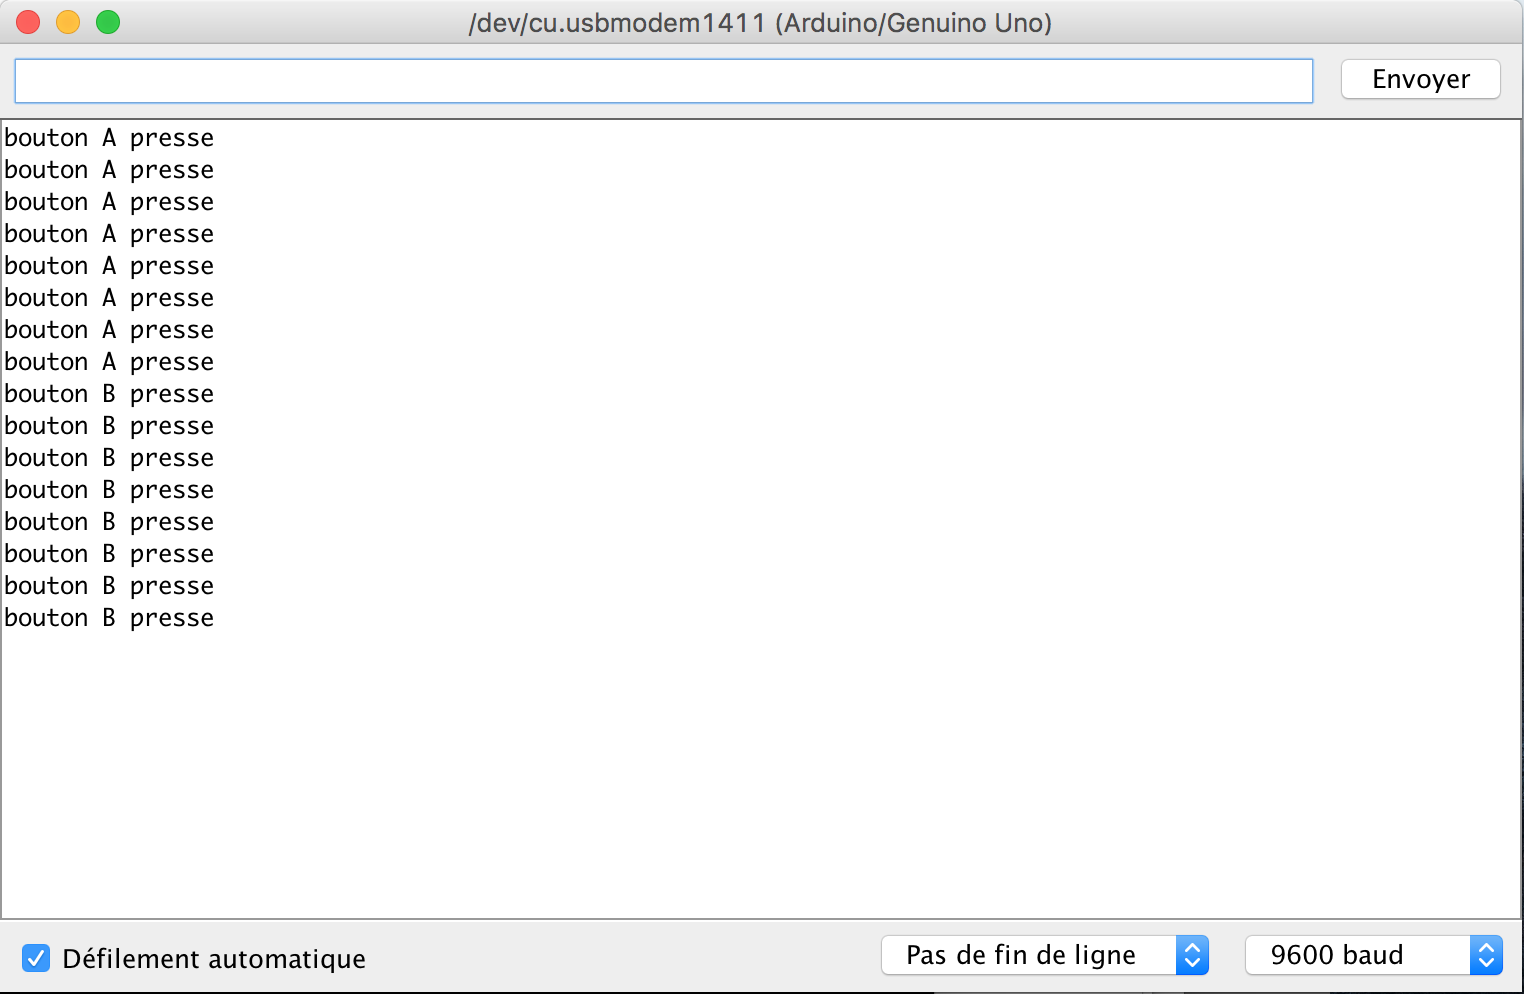
\includegraphics[width=0.75\textwidth]{terminal_serie}\\
\caption{Terminal série du logiciel arduino.}
\label{TerminalSerie}
\end{center}
\end{figure}

%}}}

\end{document}
% vim:fdl=0
